\documentclass{beamer}

\mode<presentation>
{
  \usetheme{default}
  \usecolortheme{default}
  \usefonttheme{default}
  \setbeamertemplate{navigation symbols}{}
  \setbeamertemplate{caption}[numbered]
  \setbeamertemplate{footline}[page number]
  \setbeamercolor{frametitle}{fg=white}
  \setbeamercolor{footline}{fg=black}
} 

\usepackage[english]{babel}
\usepackage[utf8x]{inputenc}
\usepackage{tikz}
\usepackage{listings}
\usepackage{courier}
\usepackage{array}
\usepackage{bold-extra}
\usepackage{minted}

\xdefinecolor{darkblue}{rgb}{0.1,0.1,0.7}
\xdefinecolor{darkgreen}{rgb}{0,0.5,0}
\xdefinecolor{darkgrey}{rgb}{0.35,0.35,0.35}
\xdefinecolor{darkorange}{rgb}{0.8,0.5,0}
\xdefinecolor{darkred}{rgb}{0.7,0,0}
\xdefinecolor{lightred}{rgb}{1,0.5,0.5}
\xdefinecolor{dianablue}{rgb}{0.18,0.24,0.31}
\definecolor{commentgreen}{rgb}{0,0.6,0}
\definecolor{stringmauve}{rgb}{0.58,0,0.82}

\lstset{ %
  backgroundcolor=\color{white},      % choose the background color
  basicstyle=\ttfamily\small,         % size of fonts used for the code
  breaklines=true,                    % automatic line breaking only at whitespace
  captionpos=b,                       % sets the caption-position to bottom
  commentstyle=\color{commentgreen},  % comment style
  escapeinside={\%*}{*)},             % if you want to add LaTeX within your code
  keywordstyle=\color{blue},          % keyword style
  stringstyle=\color{stringmauve},    % string literal style
  showstringspaces=false,
  showlines=true
}

\lstdefinelanguage{scala}{
  morekeywords={abstract,case,catch,class,def,%
    do,else,extends,false,final,finally,%
    for,if,implicit,import,match,mixin,%
    new,null,object,override,package,%
    private,protected,requires,return,sealed,%
    super,this,throw,trait,true,try,%
    type,val,var,while,with,yield},
  otherkeywords={=>,<-,<\%,<:,>:,\#,@},
  sensitive=true,
  morecomment=[l]{//},
  morecomment=[n]{/*}{*/},
  morestring=[b]",
  morestring=[b]',
  morestring=[b]"""
}

\title[2017-05-23-ecosystem-femtocode]{Femtocode: querying HEP data}
\author{Jim Pivarski}
\institute{Princeton University -- DIANA}
\date{May 23, 2017}

\begin{document}

\logo{\pgfputat{\pgfxy(0.11, 8)}{\pgfbox[right,base]{\tikz{\filldraw[fill=dianablue, draw=none] (0 cm, 0 cm) rectangle (50 cm, 1 cm);}}}\pgfputat{\pgfxy(0.11, -0.6)}{\pgfbox[right,base]{\tikz{\filldraw[fill=dianablue, draw=none] (0 cm, 0 cm) rectangle (50 cm, 1 cm);}
\includegraphics[height=0.99 cm]{diana-hep-logo.png}\tikz{\filldraw[fill=dianablue, draw=none] (0 cm, 0 cm) rectangle (4.9 cm, 1 cm);}}}}

\begin{frame}
  \titlepage
\end{frame}

\logo{\pgfputat{\pgfxy(0.11, 8)}{\pgfbox[right,base]{\tikz{\filldraw[fill=dianablue, draw=none] (0 cm, 0 cm) rectangle (50 cm, 1 cm);}
\includegraphics[height=1 cm]{diana-hep-logo.png}}}}

% Uncomment these lines for an automatically generated outline.
%\begin{frame}{Outline}
%  \tableofcontents
%\end{frame}

%%%%%%%%%%%%%%%%%%%%%%%%%%%%%%%%%%%%%%%%%%%%%%%%%%%%%%%

\begin{frame}{A data analyst's life}
\vspace{0.5 cm}
\hfill Reducing a large set of files

\hfill into a small set of files

\hfill to make plots.

\vspace{-1.5 cm}
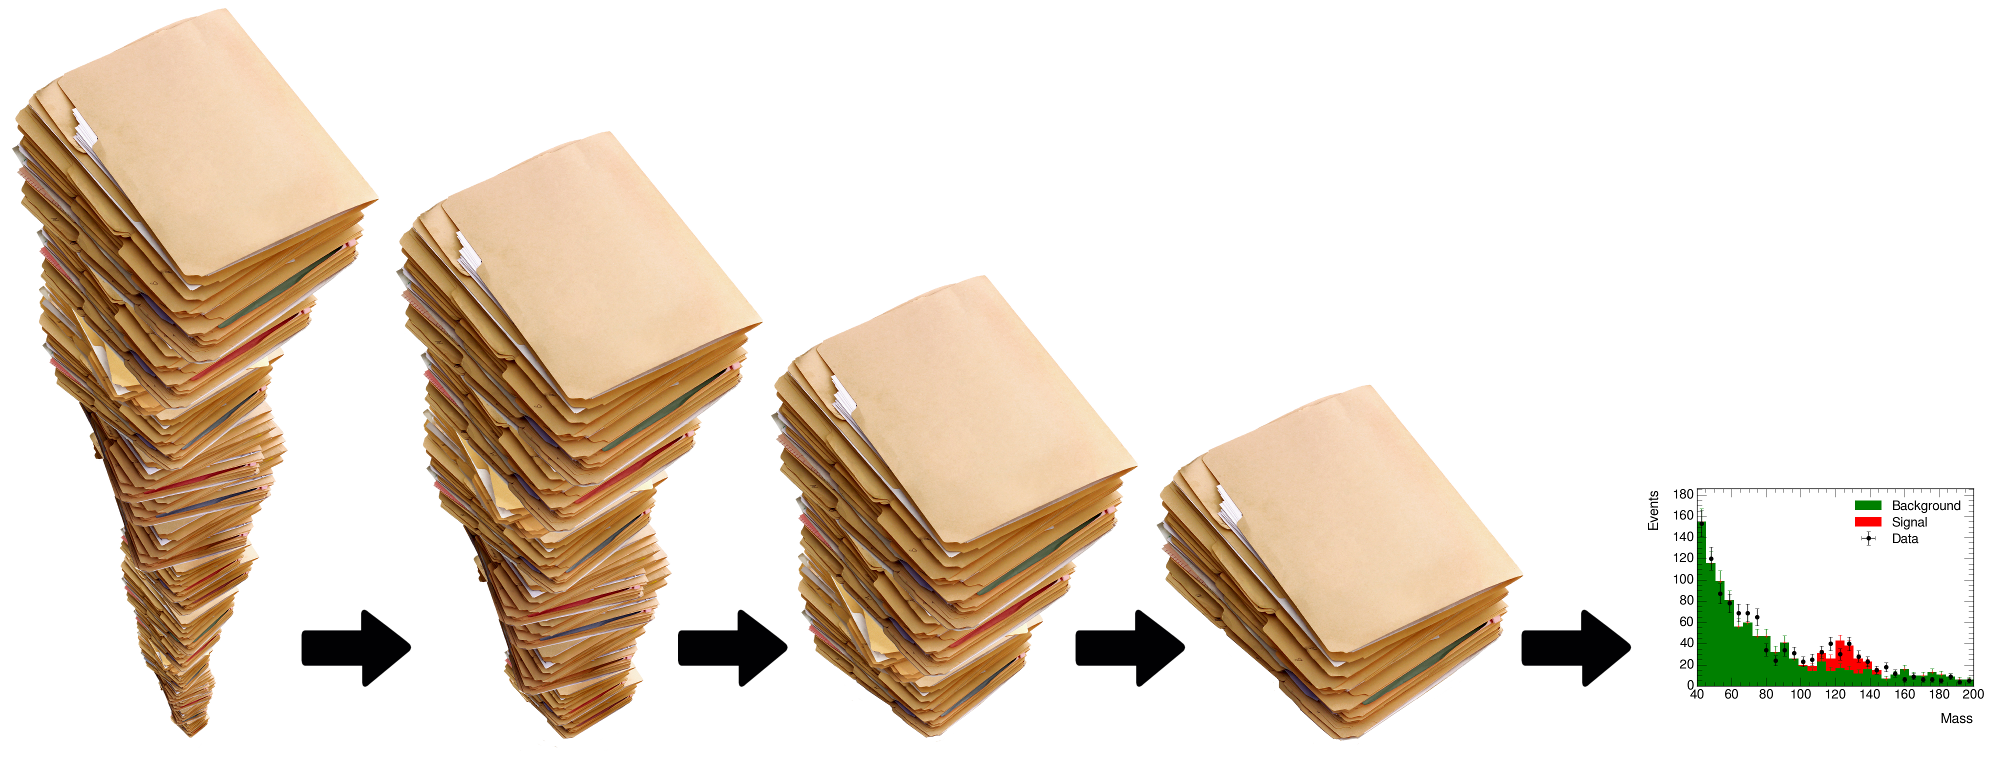
\includegraphics[width=\linewidth]{stack-of-files.png}

\vspace{0.5 cm}
The last dataset must be small enough to permit \textcolor{darkblue}{\underline{real time}} plotting and re-plotting.
\end{frame}

\begin{frame}{This is a problem}
\Large
\begin{minipage}{\linewidth}
\textcolor{darkblue}{Assertion:} if physicists {\it could} make plots \textcolor{gray}{(and other aggregations for statistical analysis)} directly from the collaboration's Analysis Object Data in real time, they {\it would.}
\end{minipage}
\end{frame}

\begin{frame}{Database-style interaction}
\vspace{0.5 cm}
\textcolor{darkblue}{Rapid queries on big data are possible; in fact, it's a big field:}

\vspace{0.5 cm}
\mbox{\hspace{-1 cm}

\includegraphics[height=1.23 cm]{sparksql-logo.png}

\includegraphics[height=1.23 cm]{impala-logo.png}

\includegraphics[height=1.23 cm]{ibis-logo.png}

\includegraphics[height=1.23 cm]{kudu-logo.png}

\includegraphics[height=1.23 cm]{hawk-logo.png}

\includegraphics[height=1.23 cm]{drill-logo.png}

\includegraphics[height=1.23 cm]{dremel-logo.png}

\includegraphics[height=1.23 cm]{bigquery-logo.png}}

\vspace{0.5 cm}
\begin{itemize}\setlength{\itemsep}{0.25 cm}
\item<2-> Instead of users maintaining private skims, running local processes, they \textcolor{darkblue}{\underline{share}} a distributed query server.
\item<3-> Instead of fetching data from disk, \textcolor{darkblue}{\underline{cache}} \mbox{in RAM/SSD/X-Point.\hspace{-1 cm}}
\item<4-> Instead of evaluating user's code as-is, \textcolor{darkblue}{\underline{translate}} it into a form that optimizes memory bandwidth.
\item<5-> Instead of executing operations on nested objects, execute on \textcolor{darkblue}{\underline{flat arrays}} of numbers.
\end{itemize}
\end{frame}

\begin{frame}{\underline{Sharing} and \underline{caching} go together}
\vspace{0.25 cm}
{\it Most} users need {\it mostly} the same input variables.
\begin{itemize}
\item For instance, all muon analyses use the same kinematic variables and might also use different isolation variables.
\item Exact fraction is unknown, but we know that analysis groups share ntuplizers that slim the same 10\% (4~kB/event) of CMS MiniAOD.
\end{itemize}

%% \vspace{0.5 cm}
%% \begin{columns}[t]
%% \column{0.5\linewidth}
%% \textcolor{darkblue}{Case 1:}

%% \textcolor{darkblue}{\underline{Users share a remote database}}

%% \vspace{0.1 cm}
%% Shared inputs are in cache once.

%% \vspace{2\baselineskip}
%% \vspace{0.1 cm}
%% Unique requirements separately cached.

%% \column{0.5\linewidth}
%% \textcolor{darkblue}{Case 2:}

%% \textcolor{darkblue}{\underline{Divide resources among users}}

%% \vspace{0.1 cm}
%% Shared inputs are separately in cache in each user's process (duplicated in different places).

%% \vspace{0.1 cm}
%% Unique requirements separately cached (same).
%% \end{columns}

\vspace{0.5 cm}
If, say, half of the variables are shared and half are not, a server distributed across a cluster with 10~TB of RAM \textcolor{darkblue}{effectively gives each user 5~TB~$+$~$\epsilon$ of RAM.}
\end{frame}

\begin{frame}{\underline{Sharing} and \underline{columnar} data go together}
\vspace{0.5 cm}
Columns for a dataset do not need to come from the same file.

\begin{center}
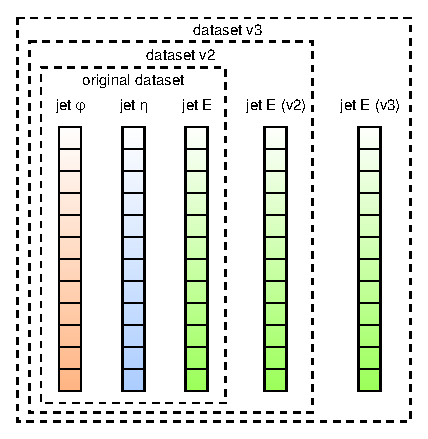
\includegraphics[width=0.6\linewidth]{virtual-datasets.pdf}
\end{center}

\vspace{-0.25 cm}
Extreme version of the ``friend TTree'' concept (superfriends).
\end{frame}

\begin{frame}{The limitation}
\mbox{\only<1>{\hspace{-0.75 cm}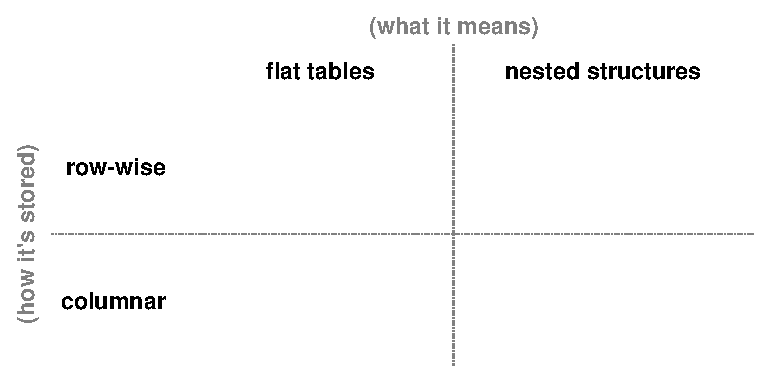
\includegraphics[width=1.15\linewidth]{table-of-formats.pdf}}\only<2>{\hspace{-0.75 cm}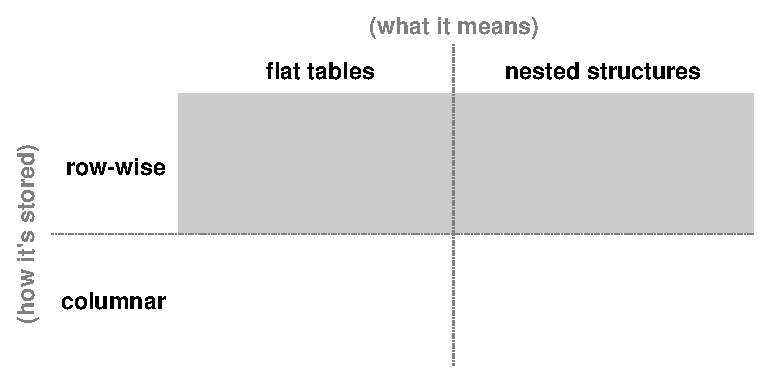
\includegraphics[width=1.15\linewidth]{table-of-formats2.pdf}}\only<3>{\hspace{-0.75 cm}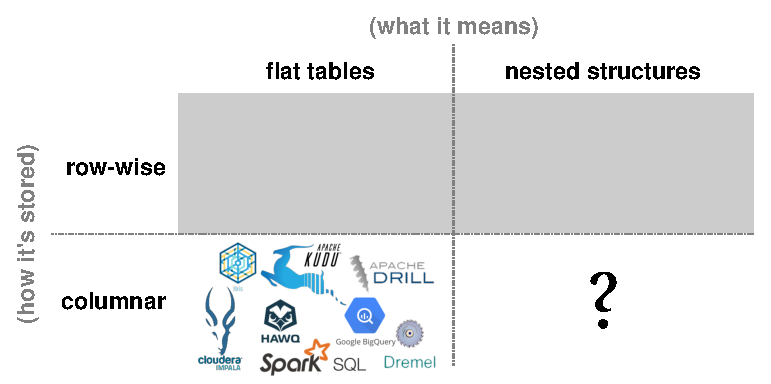
\includegraphics[width=1.15\linewidth]{table-of-formats3.pdf}}}
\end{frame}

\begin{frame}[fragile]{Femtocode: query language and engine}
\vspace{0.5 cm}
\begin{columns}[t]
\column{0.5\linewidth}
\textcolor{darkblue}{\Large \underline{Physicist's view}}

\small
\vspace{0.25 cm}
{\bf Muon object schema:}

\scriptsize
\vspace{-0.1 cm}
\begin{verbatim}
collection(record(
    pt = real(0, almost(inf)),
    eta = real,
    phi = real(-pi, pi)))
\end{verbatim}

\small
\vspace{0.25 cm}
{\bf Example query:}

\scriptsize
\begin{minted}{scala}
muons.filter(mu => mu.pt > 5)
     .map(mu => mu.pt*sinh(mu.eta))
     .max
\end{minted}

\small
\vspace{0.25 cm}
{\bf Return type:}

\scriptsize
\vspace{-0.1 cm}
\begin{verbatim}
union(null, real)
\end{verbatim}

\column{0.55\linewidth}
\textcolor{darkblue}{\Large \underline{Execution engine}}

\small
\vspace{0.25 cm}
{\bf Physical representation:}

\scriptsize
\vspace{-0.1 cm}
\begin{verbatim}
muons.pt:   [31.09, 9.76, 8.18, ...]
muons.phi:  [-0.48, 0.12, 0.12, ...]
muons.eta:  [0.88, 0.92, -0.26, ...]
muons@size: [3, 1, 1, 2, ...]
\end{verbatim}

\small
\vspace{0.25 cm}
{\bf Example execution:}

\scriptsize
\begin{enumerate}
\item Compute {\tt\scriptsize muons.pt > 5} for {\it all} muons.
\item Compute {\tt\scriptsize sinh(muons.eta)} for elements in which {\tt\scriptsize \#1} is true.
\item Compute {\tt\scriptsize muons.pt * \#2} for elements in which {\tt\scriptsize \#1} is true.
\item Pick the maximum {\tt\scriptsize \#3} value or {\tt\scriptsize NaN}, returning array with one value per event.
\end{enumerate}

\end{columns}
\end{frame}

\begin{frame}{Representing objects as flat arrays}
\vspace{0.3 cm}
For simple collections of records (e.g.\ particles), these arrays have the same interpretation as ROOT TLeaves:
\begin{itemize}
\item data arrays contain all values, ignoring event boundaries,
\item size array contains the size of each event's collection.
\end{itemize}

\vfill
\begin{uncoverenv}<2->
Except for runtime calculations, rather than just on disk.
\end{uncoverenv}

\vfill
\begin{uncoverenv}<3->
For collections of collections (with fixed, known depth), we can extend this definition recursively:

\vspace{0.3 cm}
\textcolor{darkblue}{Given:} \hfill {\tt [} {\tt [} {\tt a} {\tt b} {\tt c} {\tt ]} {\tt [} {\tt d} {\tt e} {\tt f} {\tt g} {\tt ]} {\tt ]} {\tt [} {\tt [} {\tt h} {\tt ]} {\tt [} {\tt i} {\tt j} {\tt ]} {\tt ]}

\textcolor{darkblue}{Data array:} \hfill {\tt \ } {\tt \ } {\tt a} {\tt b} {\tt c} {\tt \ } {\tt \ } {\tt d} {\tt e} {\tt f} {\tt g} {\tt \ } {\tt \ } {\tt \ } {\tt \ } {\tt h} {\tt \ } {\tt \ } {\tt i} {\tt j} {\tt \ } {\tt \ }

\textcolor{darkblue}{Recursive counter:} \hfill \textcolor{darkorange}{\tt 2} \textcolor{blue}{\tt 3} {\tt \ } {\tt \ } {\tt \ } {\tt \ } \textcolor{blue}{\tt 4} {\tt \ } {\tt \ } {\tt \ } {\tt \ } {\tt \ } {\tt \ } \textcolor{darkorange}{\tt 2} \textcolor{blue}{\tt 1} {\tt \ } {\tt \ } \textcolor{blue}{\tt 2} {\tt \ } {\tt \ } {\tt \ } {\tt \ }
\end{uncoverenv}
\end{frame}

\begin{frame}{Granular unit of parallelization}
\vspace{0.5 cm}
\begin{columns}
\column{0.5\linewidth}
\large
Each query might touch any column, so the unit of parallelization is an group of columns with an integer number of events.
\column{0.5\linewidth}
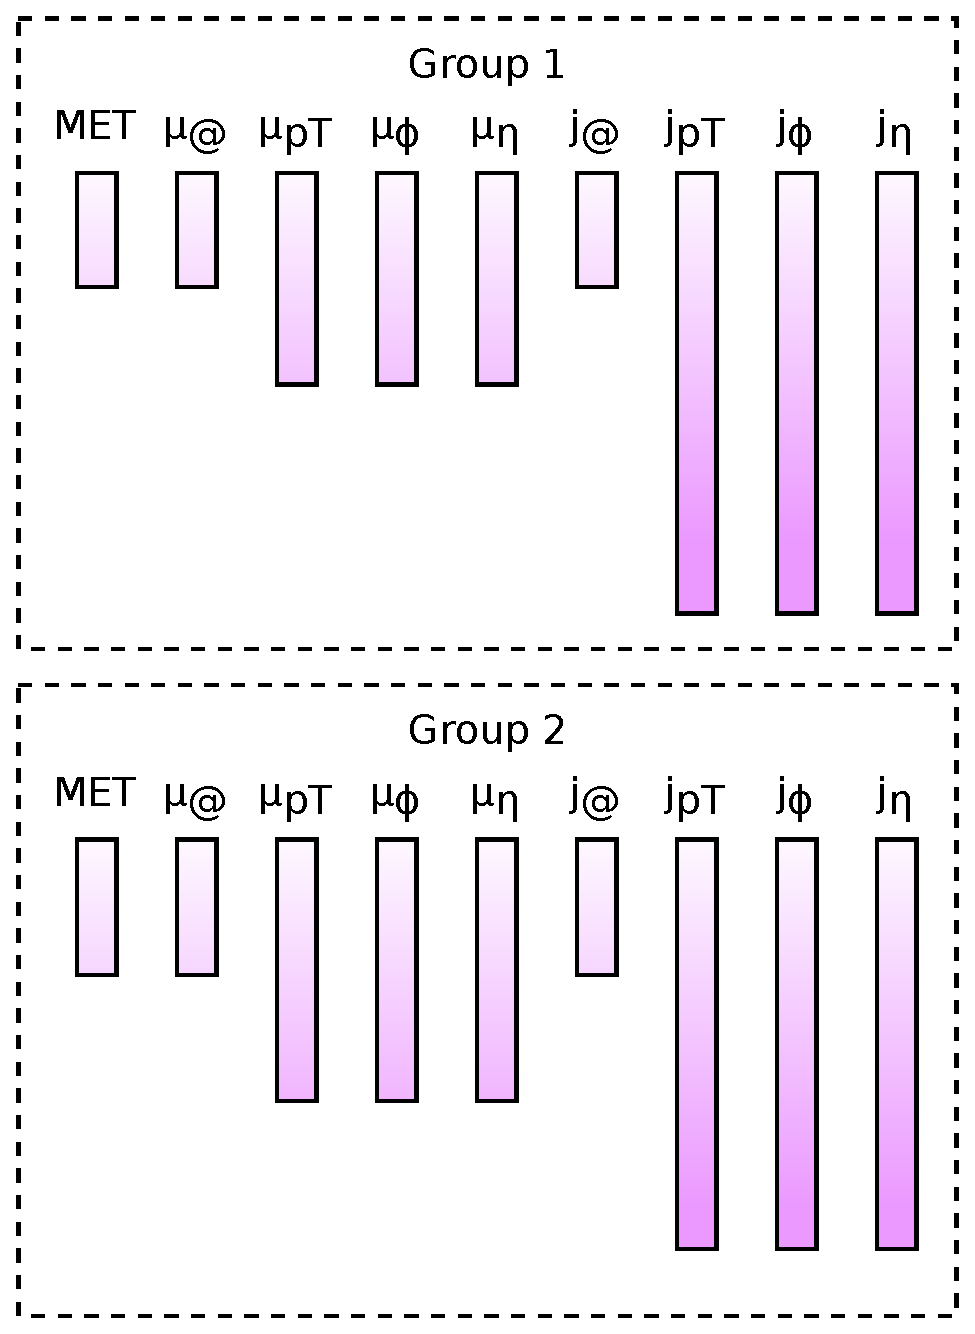
\includegraphics[width=\linewidth]{groups.pdf}
\end{columns}
\end{frame}

\begin{frame}{Query system layout}
\vspace{0.15 cm}
\mbox{\hspace{-1.1 cm}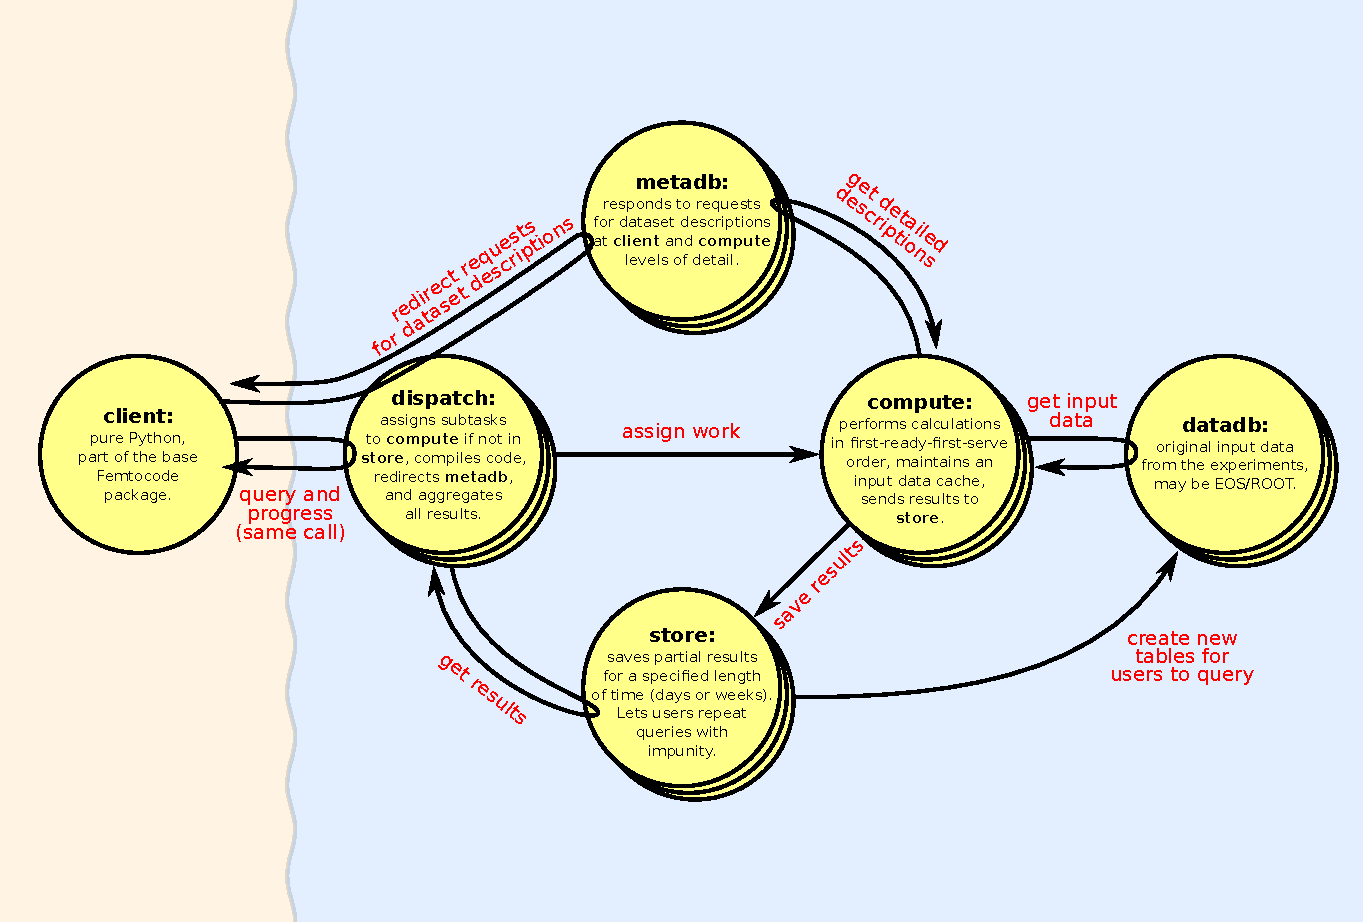
\includegraphics[width=1.2\linewidth]{distributed-system-tall.pdf}}
\end{frame}

\begin{frame}[fragile]{Working example: dimuons}
\vspace{0.15 cm}
\scriptsize
\begin{Verbatim}[commandchars=\\\{\}]
pending = session.\textcolor{blue}{source}(\textcolor{red}{"ZZ_13TeV_pythia8"})
    .\textcolor{blue}{define}(\textcolor{darkgreen}{mumass} = \textcolor{red}{"0.105658"})     \textcolor{gray}{# chain of operations on source}
    .\textcolor{blue}{toPython}(\textcolor{darkgreen}{mass} = \textcolor{red}{"""}
\textcolor{red}{muons.map(mu1 => muons.map(\{mu2 =>}   \textcolor{gray}{# doubly nested loop over muons}
\textcolor{red}{  p1x = mu1.pt * cos(mu1.phi);}
\textcolor{red}{  p1y = mu1.pt * sin(mu1.phi);}       \textcolor{gray}{# shares scope with other steps}
\textcolor{red}{  p1z = mu1.pt * sinh(mu1.eta);}      \textcolor{gray}{# in the chain (see "mumass")}
\textcolor{red}{  E1 = sqrt(p1x**2 + p1y**2 + p1z**2 + mumass**2);}

\textcolor{red}{  p2x = mu2.pt * cos(mu2.phi);}
\textcolor{red}{  p2y = mu2.pt * sin(mu2.phi);}
\textcolor{red}{  p2z = mu2.pt * sinh(mu2.eta);}
\textcolor{red}{  E2 = sqrt(p2x**2 + p2y**2 + p2z**2 + mumass**2);}

\textcolor{red}{  px = p1x + p2x; py = p1y + p2y;}
\textcolor{red}{  pz = p1z + p2z; E = E1 + E2;}

\textcolor{gray}{  # "if" is required to avoid sqrt(-x)}
\textcolor{red}{  if E**2 - px**2 - py**2 - pz**2 >= 0:}
\textcolor{red}{    sqrt(E**2 - px**2 - py**2 - pz**2)}
\textcolor{red}{  else:}
\textcolor{red}{    None}   \textcolor{gray}{# output type is nullable}
\textcolor{red}{\}))}
\textcolor{red}{"""}).\textcolor{blue}{submit}()                        \textcolor{gray}{# asynchronous submission to}
final = pending.\textcolor{blue}{await}()              \textcolor{gray}{# watch result accumulate}
\end{Verbatim}

\vspace{-4 cm}
\hfill \textcolor{gray}{Yes, we see the Z peak.\hspace{0.25 cm}}

\vspace{-0.2 cm}
\hfill \mbox{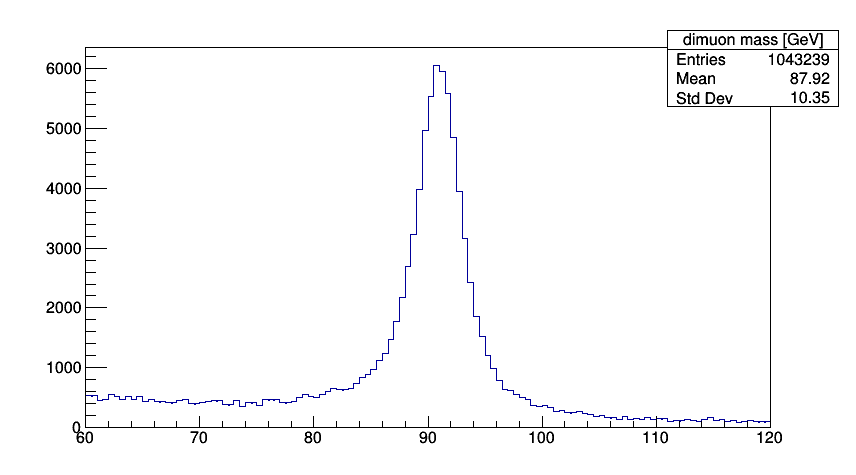
\includegraphics[width=0.48\linewidth]{c1.png}\hspace{-1 cm}}
\vspace{4 cm}
\end{frame}

\begin{frame}{Comparing apples and bananas}
\vspace{0.5 cm}
\textcolor{darkblue}{\underline{I/O-bounded operation (plus) on 806\,177 jet $p_T$ values (6.15 MB):}}

\vspace{-0.4 cm}
\begin{center}
\renewcommand{\arraystretch}{1.2}
\small
\begin{tabular}{r l}
0.018 MHz & CMSSW EDAnalyzer (too many branches loaded) \\
1.5 MHz & {\tt TTree::Draw} into single-bin histogram \\
2.8 MHz & minimal disk read and unzip (ROOT or Numpy) \\
12 MHz & allocating C++ objects on heap, iterating, deleting \\
31 MHz & allocating C++ objects on stack, iterating \\
\textcolor{darkblue}{54 MHz} & \textcolor{darkblue}{current implementation of Femtocode loop$^*$} \\
250 MHz & minimal single-threaded loop in C (our goal) \\
8\,000 MHz & same loop on 128 threads in KNL's MCDRAM \\
57\,000 MHz & equivalent on Tesla P100-SXM2 GPU \\
\end{tabular}
\end{center}

\vspace{0.5 cm}
\textcolor{darkblue}{$^*$Not final.}
\end{frame}

\begin{frame}{Concluding remarks}
\begin{center}
\Large
Shared query-based data access is worth pursuing.

\vspace{0.5 cm}
Femtocode is an implementation of that idea, \\ and is starting to work.
\end{center}
\end{frame}

\begin{frame}[fragile]{Taking this example apart (1/3)}
\vspace{0.25 cm}
\begin{itemize}
\item Femtocode always appears in quotes (like SQL). It is a big-data aggregation step that feeds into a traditional analysis.

\item A query is a ``workflow'' from source to aggregation, compiled and submitted as one unit.

e.g.\ {\tt\scriptsize \textcolor{blue}{source}(\textcolor{red}{"dataset"}).\textcolor{blue}{define}(X).\textcolor{blue}{define}(Y).\textcolor{blue}{histogrammar}(Z) }

\item Most Femtocode snippets are tiny (hence ``femto''), scattered throughout a Histogrammar aggregation:

\scriptsize
\begin{Verbatim}[commandchars=\\\{\}]
session.\textcolor{blue}{source}(\textcolor{red}{"dataset"})
    .\textcolor{blue}{define}(\textcolor{darkgreen}{goodmuons} = \textcolor{red}{"""..."""})  \textcolor{gray}{# define good muons}
    .\textcolor{blue}{filter}(\textcolor{red}{"goodmuons.size >= 2"})  \textcolor{gray}{# cut on them}
    .\textcolor{blue}{define}(\textcolor{darkgreen}{dimuon} = \textcolor{red}{"""..."""}      \textcolor{gray}{# define dimuons}
    .\textcolor{blue}{bundle}(                        \textcolor{gray}{# plot their attributes}
        \textcolor{darkgreen}{mass} = \textcolor{blue}{bin}(120, 0, 12, \textcolor{red}{"dimuon.mass"}),
        \textcolor{darkgreen}{pt} = \textcolor{blue}{bin}(100, 0, 100, \textcolor{red}{"dimuon.pt"}),
        \textcolor{darkgreen}{eta} = \textcolor{blue}{bin}(100, -5, 5, \textcolor{red}{"dimuon.eta"}),
        \textcolor{darkgreen}{phi} = \textcolor{blue}{bin}(314, 0, 2*pi, \textcolor{red}{"dimuon.phi + pi"}),
                                    \textcolor{gray}{# also plot the muons}
        \textcolor{darkgreen}{muons} = \textcolor{blue}{loop}(\textcolor{red}{"goodmuons"}, \textcolor{red}{"mu"}, bundle(
            \textcolor{darkgreen}{pt} = \textcolor{blue}{bin}(100, 0, 100, \textcolor{red}{"mu.pt"}),
            \textcolor{darkgreen}{eta} = \textcolor{blue}{bin}(100, -5, 5, \textcolor{red}{"mu.eta"}),
            \textcolor{darkgreen}{phi} = \textcolor{blue}{bin}(314, -pi, pi, \textcolor{red}{"mu.phi"}))))
\end{Verbatim}
\end{itemize}
\end{frame}

\begin{frame}[fragile]{Taking this example apart (2/3)}
\vspace{0.3 cm}
\begin{itemize}\setlength{\itemsep}{0.5 cm}
\item Loop over pairs of muons is constructed by \mbox{nesting functionals:\hspace{-1 cm}}

\mbox{\tt\small \textcolor{red}{"muons.map(mu1 => muons.map(mu2 => f(mu1, mu2)))"}\hspace{-1 cm}}

is equivalent to

\begin{center}
\begin{minipage}{0.7\linewidth}
\scriptsize
\begin{minted}{python}
list_of_lists = []
for mu1 in muons:
    list_of_numbers = []
    for mu2 in muons:
        list_of_numbers.append(f(mu1, mu2))
    list_of_lists.append(list_of_numbers)

return list_of_lists
\end{minted}
\end{minipage}
\end{center}

\item There will someday be more convenient forms: \textcolor{red}{\tt pairs}, \textcolor{red}{\tt table}, \textcolor{red}{\tt filter}, \textcolor{red}{\tt flatten}, \textcolor{red}{\tt flatMap}, \textcolor{red}{\tt zip}, \textcolor{red}{\tt permutations}, etc.

\vspace{0.2 cm}
\textcolor{gray}{(The dimuon example would ideally use \textcolor{lightred}{\tt pairs} to avoid double-counting and \textcolor{lightred}{\tt flatten} to destructure the list-of-lists. Or better yet, pick two by $p_T$ to get one candidate per event.)}
\end{itemize}
\end{frame}

\begin{frame}[fragile]{Taking this example apart (3/3)}
\vspace{0.2 cm}
\begin{itemize}
\item Type system requires domain of \textcolor{red}{\tt sqrt} to be guarded:

\scriptsize
\begin{Verbatim}[commandchars=\\\{\}]
  \textcolor{red}{sqrt(E**2 - px**2 - py**2 - pz**2)}

FemtocodeError: Function "sqrt" does not accept arguments with
the given types:

    sqrt(real)

    The sqrt function can only be used on non-negative numbers.

Check line:col 19:2 (pos 401):
      sqrt(E**2 - px**2 - py**2 - pz**2)
------^
\end{Verbatim}

\vspace{0.1 cm}
\normalsize To resolve this compile-time error, we write:

\scriptsize
\begin{Verbatim}[commandchars=\\\{\}]
  \textcolor{red}{if E**2 - px**2 - py**2 - pz**2 >= 0:}
  \textcolor{red}{    sqrt(E**2 - px**2 - py**2 - pz**2)}
  \textcolor{red}{else:}
  \textcolor{red}{    None}
\end{Verbatim}

\normalsize

\item The compiler tracks each subexpression's interval of validity: \textcolor{red}{\tt\scriptsize E**2 - px**2 - py**2 - pz**2} is limited to \mbox{{\tt\scriptsize real(min=0, max=inf)}.\hspace{-1 cm}}

\vspace{0.2 cm}
In the future, we could use SymPy to discover \mbox{this algebraically.\hspace{-1 cm}}
\end{itemize}
\end{frame}

\begin{frame}{Another thing to notice}
\[
\begin{array}{ll}
\mbox{\textcolor{red}{\tt\scriptsize muons.map(mu1 => muons.map(\{mu2 =>}} & \\

\left.\renewcommand{\arraystretch}{0.7}\begin{array}{p{8 cm}}
\mbox{\textcolor{red}{\tt\scriptsize p1x = mu1.pt * cos(mu1.phi);}} \\
\mbox{\textcolor{red}{\tt\scriptsize p1y = mu1.pt * sin(mu1.phi);}} \\
\mbox{\textcolor{red}{\tt\scriptsize p1z = mu1.pt * sinh(mu1.eta);}} \\
\mbox{\textcolor{red}{\tt\scriptsize E1 = sqrt(p1x**2 + p1y**2 + p1z**2 + mumass**2);}}
\end{array}\right\} &
\mbox{only uses \textcolor{red}{\tt mu1}} \\
& \\
\left.\renewcommand{\arraystretch}{0.7}\begin{array}{p{8 cm}}
\mbox{\textcolor{red}{\tt\scriptsize p2x = mu2.pt * cos(mu2.phi);}} \\
\mbox{\textcolor{red}{\tt\scriptsize p2y = mu2.pt * sin(mu2.phi);}} \\
\mbox{\textcolor{red}{\tt\scriptsize p2z = mu2.pt * sinh(mu2.eta);}} \\
\mbox{\textcolor{red}{\tt\scriptsize E2 = sqrt(p2x**2 + p2y**2 + p2z**2 + mumass**2);}}
\end{array}\right\} &
\mbox{only uses \textcolor{red}{\tt mu2}} \\
& \\
\left.\renewcommand{\arraystretch}{0.7}\begin{array}{p{8 cm}}
\mbox{\textcolor{red}{\tt\scriptsize px = p1x + p2x;}} \\
\mbox{\textcolor{red}{\tt\scriptsize py = p1y + p2y;}} \\
\mbox{\textcolor{red}{\tt\scriptsize pz = p1z + p2z;}} \\
\mbox{\textcolor{red}{\tt\scriptsize E = E1 + E2;}} \\
\mbox{\textcolor{red}{\tt\scriptsize }} \\
\mbox{\textcolor{red}{\tt\scriptsize if E**2 - px**2 - py**2 - pz**2 >= 0:}} \\
\mbox{\textcolor{red}{\tt\scriptsize \hspace{0.25 cm}sqrt(E**2 - px**2 - py**2 - pz**2)}} \\
\mbox{\textcolor{red}{\tt\scriptsize else:}} \\
\mbox{\textcolor{red}{\tt\scriptsize \hspace{0.25 cm}None}}
\end{array}\right\} &
\mbox{uses both.} \\
\mbox{\textcolor{red}{\tt\scriptsize \}))}} & \\
\end{array}
\]
\end{frame}

\begin{frame}[fragile]{The dimuon example, after ``compilation''}
\vspace{-0.2 cm}
\begin{columns}[t]
\column{0.5\linewidth}
\tiny
\begin{Verbatim}[commandchars=\\\{\}]
Sized by muons[]@size:
    #0       := \textcolor{red}{cos}(muons[]-phi)
    #1       := \textcolor{red}{*}(muons[]-pt, #0)
    #2       := \textcolor{red}{**}(#1, \textcolor{darkgreen}{2})
    #3       := \textcolor{red}{sin}(muons[]-phi)
    #4       := \textcolor{red}{*}(muons[]-pt, #3)
    #5       := \textcolor{red}{**}(#4, \textcolor{darkgreen}{2})
    #6       := \textcolor{red}{sinh}(muons[]-eta)
    #7       := \textcolor{red}{*}(muons[]-pt, #6)
    #8       := \textcolor{red}{**}(#7, \textcolor{darkgreen}{2})
    #9       := \textcolor{red}{+}(#2, #5, #8, \textcolor{darkgreen}{0.011164})
    #10      := \textcolor{red}{sqrt}(#9)
\textcolor{gray}{type(#10) == real(0.105658, almost(inf))}

Sized by \#11@size:
    #11@size := \textcolor{red}{$explodesize}(muons[], muons[])
    #11      := \textcolor{red}{$explodedata}(#10, #11@size, (muons[]))
    #12      := \textcolor{red}{$explodedata}(#10, #11@size, (muons[], muons[]))
    #13      := \textcolor{red}{+}(#11, #12)
    #14      := \textcolor{red}{**}(#13, \textcolor{darkgreen}{2})
    #15      := \textcolor{red}{$explodedata}(#1, #11@size, (muons[]))
    #16      := \textcolor{red}{$explodedata}(#1, #11@size, (muons[], muons[]))
    #17      := \textcolor{red}{+}(#15, #16)
    #18      := \textcolor{red}{**}(#17, \textcolor{darkgreen}{2})
    #19      := \textcolor{red}{-}(#14, #18)
    #20      := \textcolor{red}{$explodedata}(#4, #11@size, (muons[]))
    #21      := \textcolor{red}{$explodedata}(#4, #11@size, (muons[], muons[]))
    #22      := \textcolor{red}{+}(#20, #21)
    #23      := \textcolor{red}{**}(#22, \textcolor{darkgreen}{2})
    #24      := \textcolor{red}{-}(#19, #23)
    #25      := \textcolor{red}{$explodedata}(#7, #11@size, (muons[]))
    #26      := \textcolor{red}{$explodedata}(#7, #11@size, (muons[], muons[]))
\end{Verbatim}

\column{0.5\linewidth}
\tiny
\begin{Verbatim}[commandchars=\\\{\}]

    #27      := \textcolor{red}{+}(#25, #26)
    #28      := \textcolor{red}{**}(#27, \textcolor{darkgreen}{2})
    #29      := \textcolor{red}{-}(#24, #28)
    #30      := \textcolor{red}{>=}(#29, \textcolor{darkgreen}{0})
    #31      := \textcolor{red}{<}(#29, \textcolor{darkgreen}{0})
    #32      := \textcolor{red}{-}(#24, #28)
    #33      := \textcolor{red}{sqrt}(#32)
    #34      := \textcolor{red}{if}(#30, #31, #33, \textcolor{darkgreen}{None})
\textcolor{gray}{type(#34) == union(null, real(0, almost(inf)))}
\end{Verbatim}

\vspace{0.3 cm}
\hfill \fbox{\begin{minipage}{2.6 cm}
\scriptsize\raggedright {\tt muons[]-pt}, {\tt muons[]-phi}, {\tt muons[]-eta}, {\tt muons[]@size}, and everything that starts with a {\tt \#} is (at least conceptually) a big array of values.

\vspace{0.2 cm}
All functions except \textcolor{red}{\tt \$explode*} would make good GPU kernels.
\end{minipage}}
\end{columns}
\end{frame}

\begin{frame}{Freedom to choose the looping structure}
\vspace{0.2 cm}
\only<1>{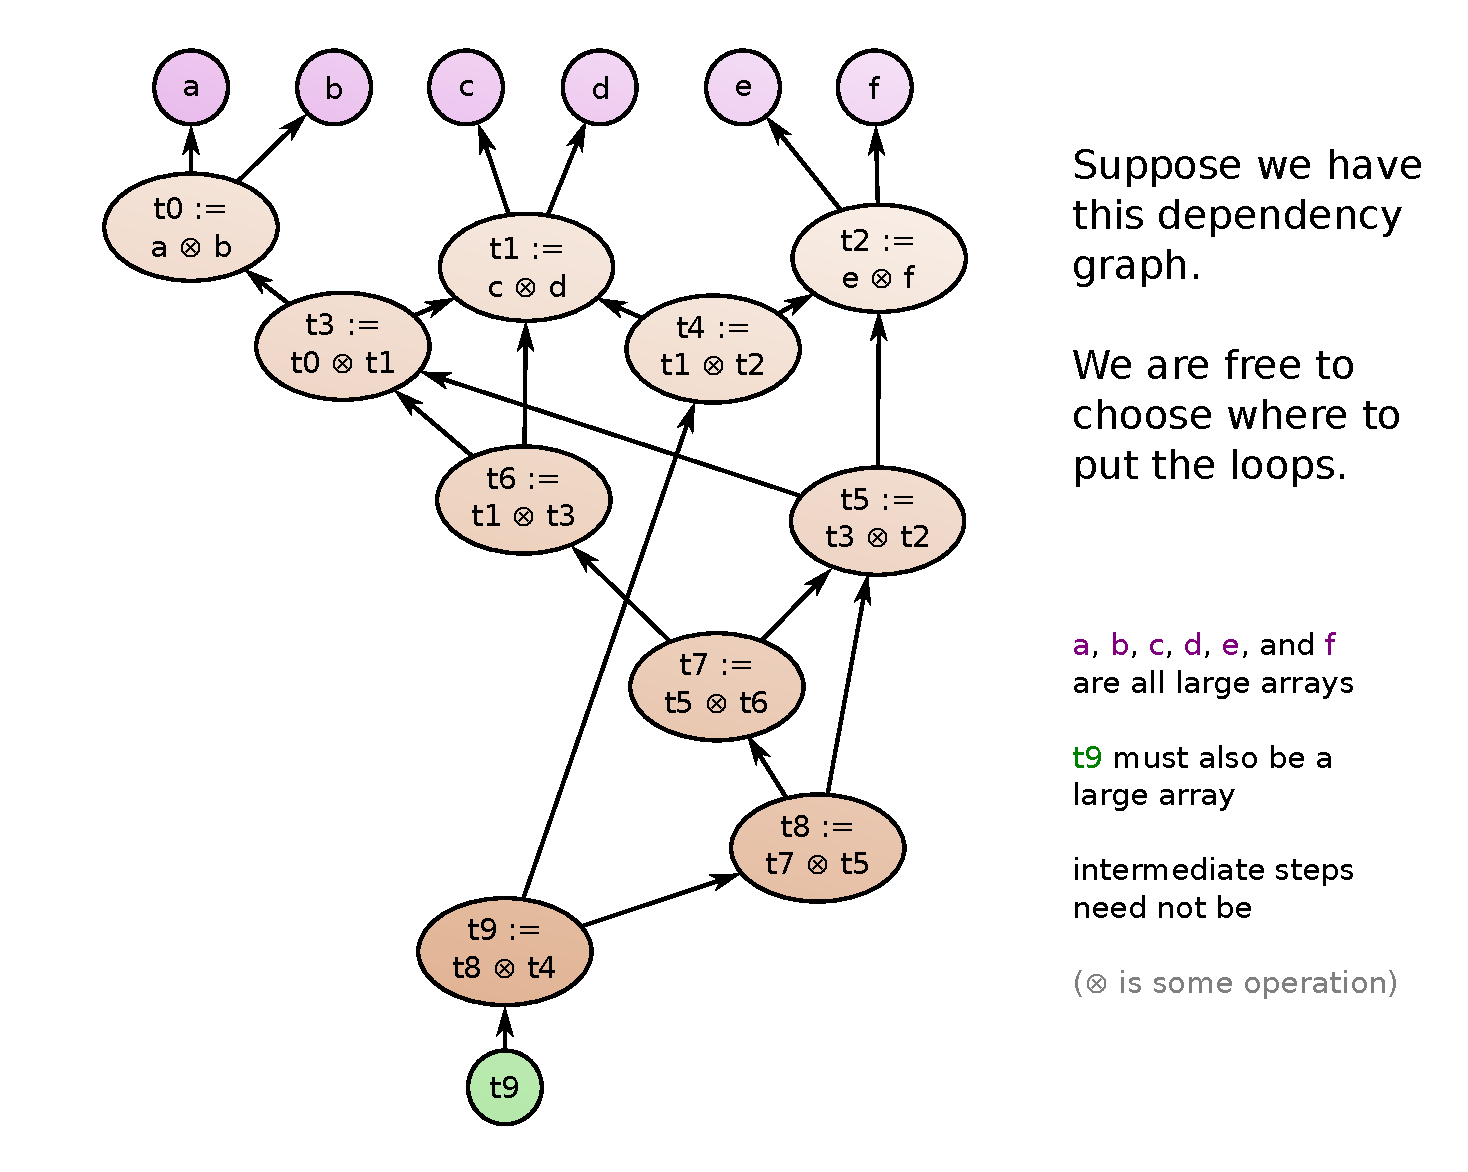
\includegraphics[width=\linewidth]{dependencygraph.pdf}}
\only<2>{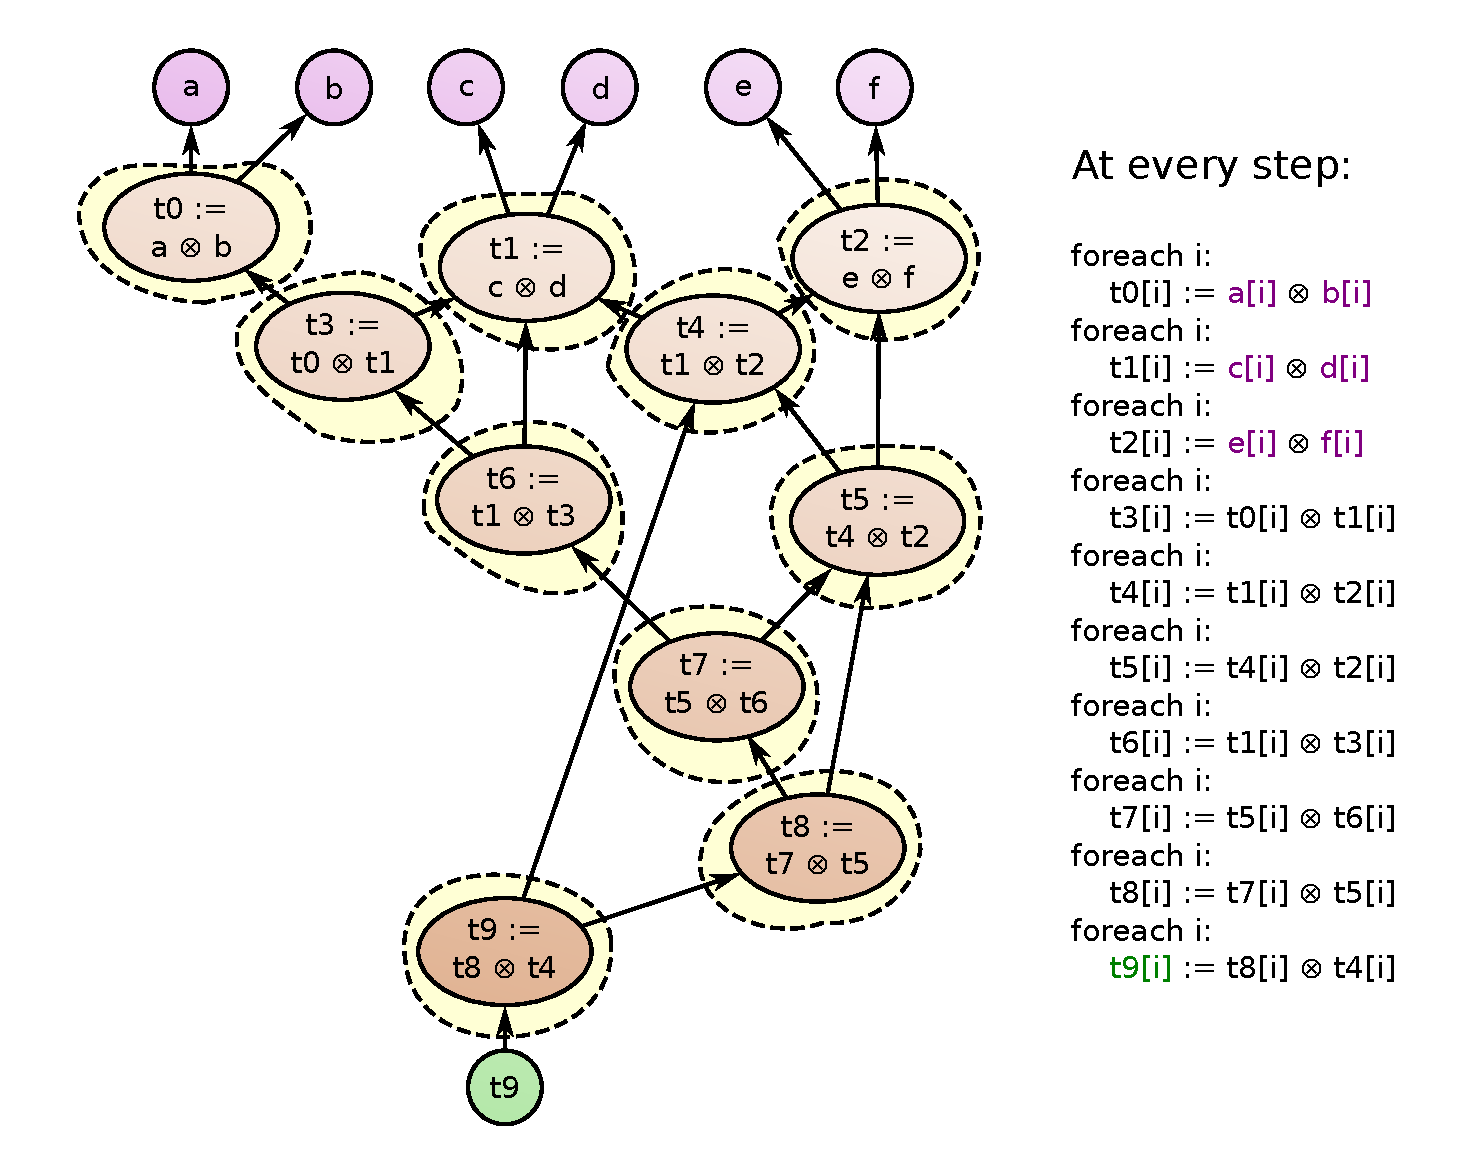
\includegraphics[width=\linewidth]{dependencygraph_1.pdf}}
\only<3>{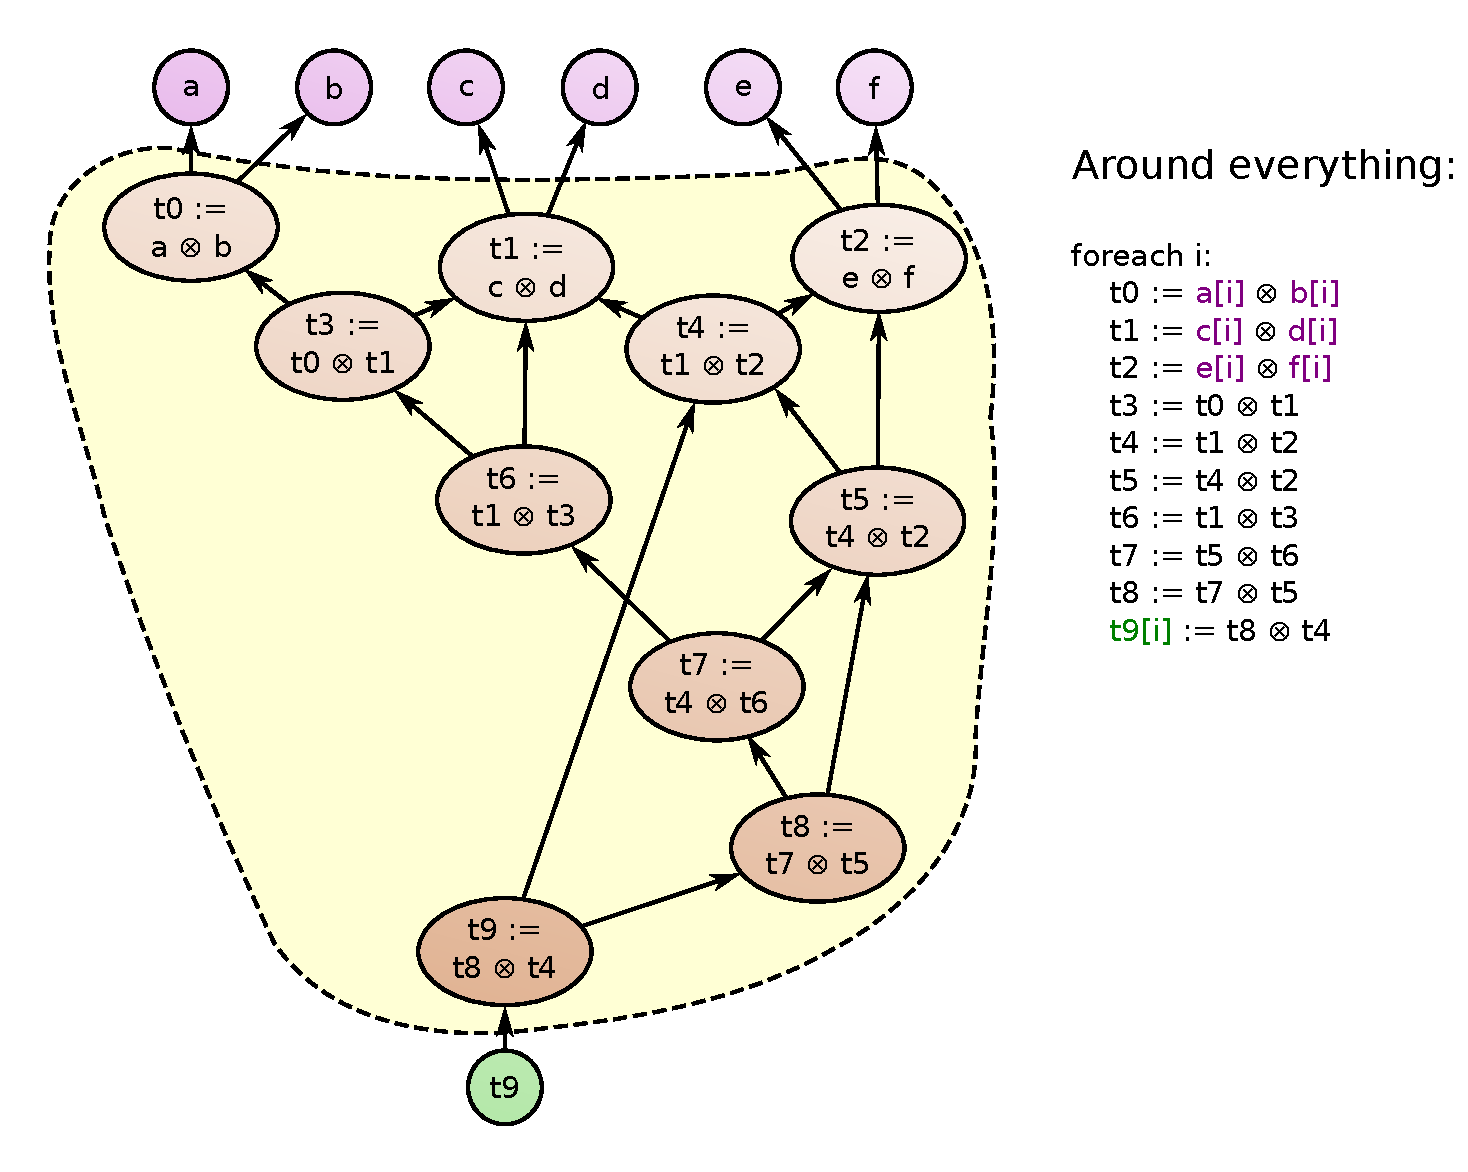
\includegraphics[width=\linewidth]{dependencygraph_2.pdf}}
\only<4>{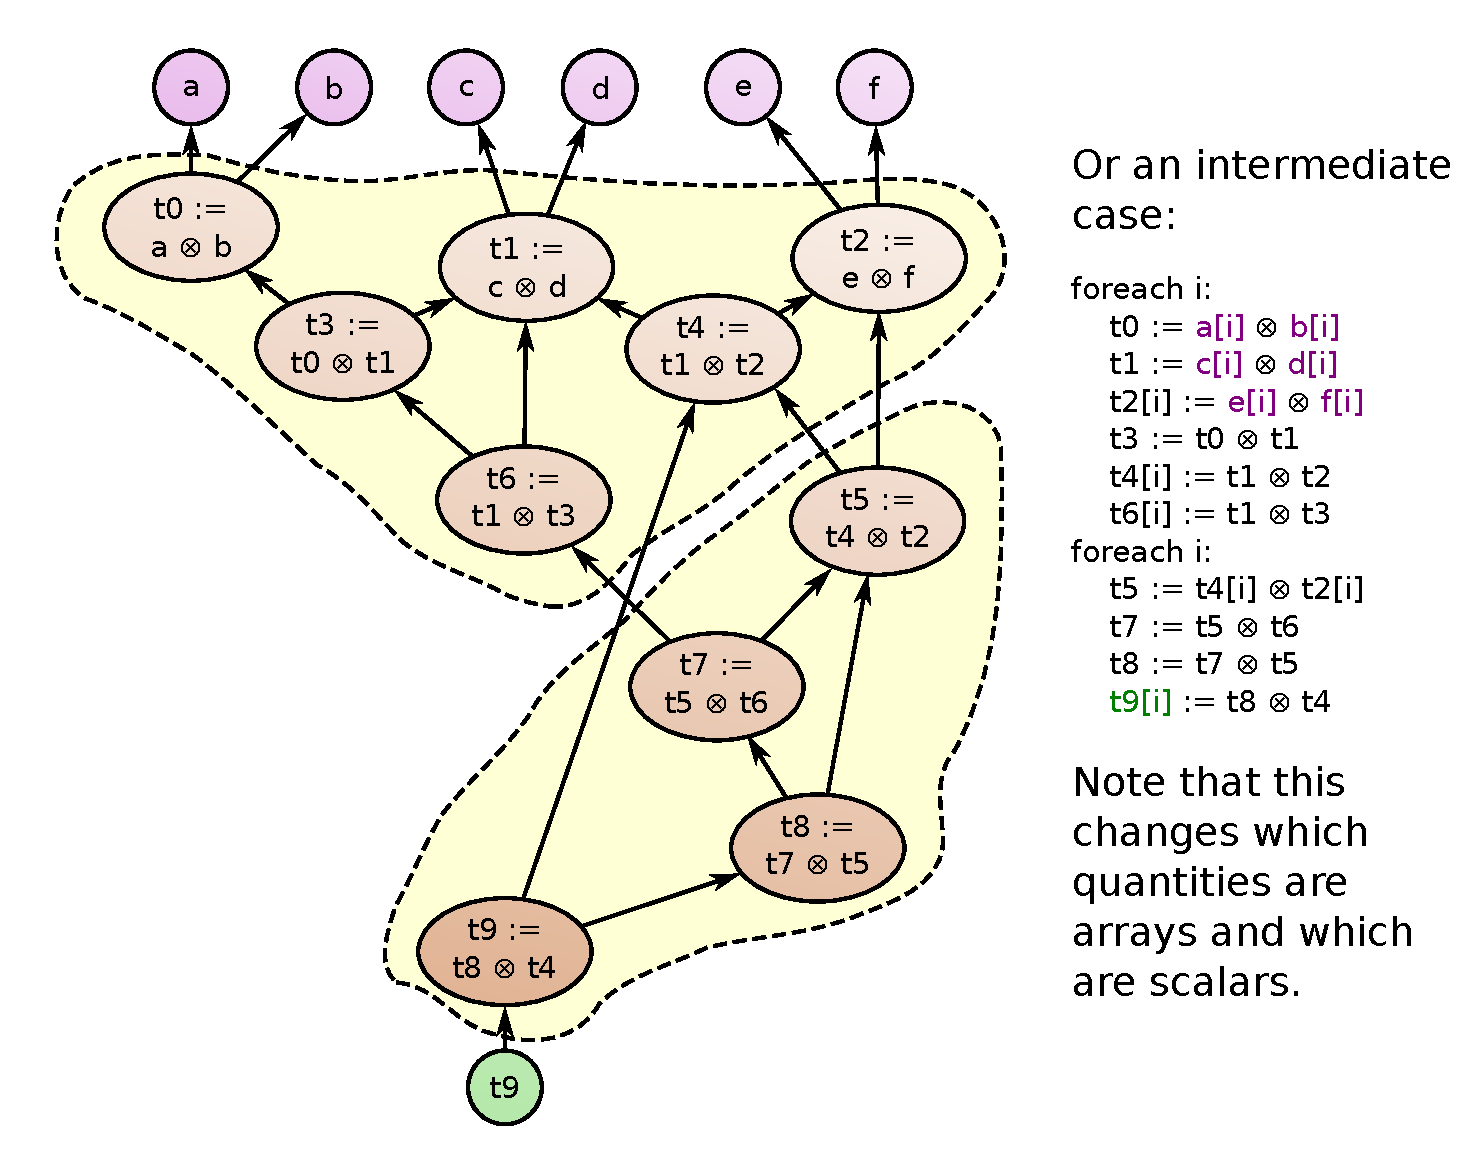
\includegraphics[width=\linewidth]{dependencygraph_3.pdf}}
\end{frame}

\begin{frame}{Three kinds of operations in each plateau}
\mbox{\hspace{-0.5 cm}\begin{minipage}{1.1\linewidth}
\begin{description}\setlength{\itemsep}{0.75 cm}
\item[Explode:] increase cardinality of one array \\ so that it matches another. \\ Determines the indexing of the \\ loop, so must be first.

\vspace{-4\baselineskip}
\hfill 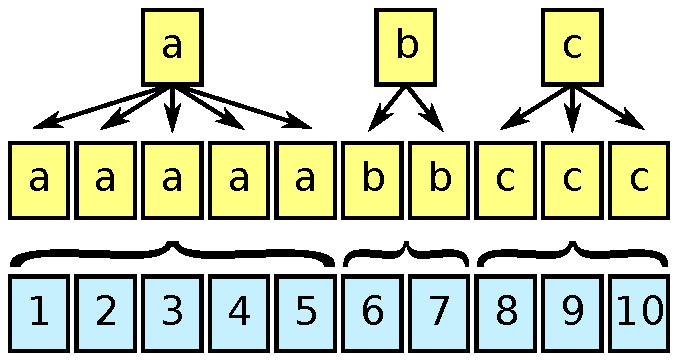
\includegraphics[width=0.37\linewidth]{explode.pdf}

\item[Flat:] apply function to all members of \\ two aligned data arrays, ignoring \\ event boundaries. Intermediate \\ steps need not be arrays.

\vspace{-4\baselineskip}
\hfill 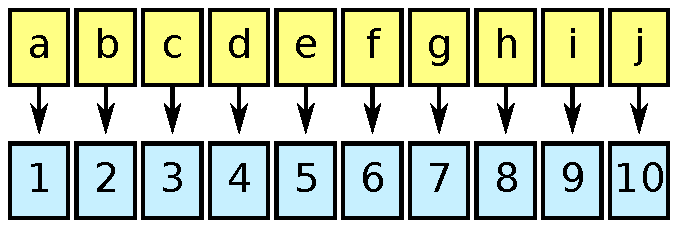
\includegraphics[width=0.37\linewidth]{flat.pdf}

\vspace{0.3 cm}
\item[Implode:] combine results (sum, mean, max, \\ etc.) to reduce cardinality of an \\ array. Size of output arrays are not \\ constrained by the indexing of the \\ loop. Must be last.

\vspace{-5\baselineskip}
\hfill 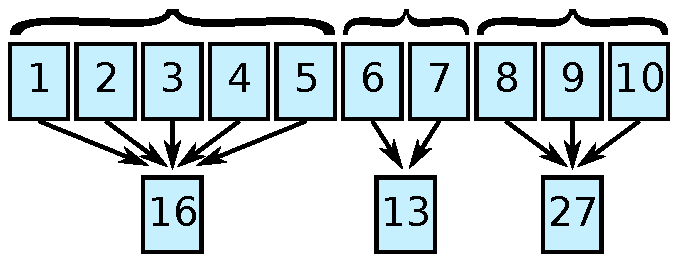
\includegraphics[width=0.37\linewidth]{implode.pdf}
\end{description}
\end{minipage}}
\end{frame}

\begin{frame}[fragile]{Using ROOT functions in Femtocode}
\vspace{0.1 cm}
\tiny
\begin{minted}[frame=single]{python}
########## ROOT/some_library.py, somewhere visible to nodes on the Femtocode server.
import ctypes
libMathCore = ctypes.cdll.LoadLibrary("libMathCore.so")
chi2_ctypes = libMathCore._ZN5TMath17ChisquareQuantileEdd    # c++filt!
chi2_ctypes.argtypes = (ctypes.c_double, ctypes.c_double)
chi2_ctypes.restype = ctypes.c_double
\end{minted}

\begin{minted}[frame=single]{python}
########## Creating a custom library (on the Femtocode client):
from femtocode.typesystem import *
from femtocode.lib.custom import *

def chi2_sig(x, n):
    # Compile-time type-safety: assert parameter types, provide return type.
    assert isinstance(x, Number) and \
        almost.min(0, x.min) == 0 and almost.max(x.max, almost(1)) == almost(1)
    assert isinstance(n, Number) and n.whole and n.min > 0
    return real(0, almost(inf))

custom = CustomLibrary()            # module name          symbol name    signature
custom.add(CustomFlatFunction("chi2", "ROOT.some_library", "chi2_ctypes", chi2_sig))

########## Running a Femtocode query that uses this library:
from femtocode.run.execution import NativeTestSession
session = NativeTestSession()

# Define a dataset with the right types and fill it with dummy data.
numerical = session.source("Test", x=real(0, almost(1)), n=integer(1, almost(inf)))
for i in range(100):
    numerical.dataset.fill({"x": i / 100.0, "n": i + 1})

# Femtocode calls TMath::ChisquareQuantile without involving Python at all.
result = numerical.toPython(out = "chi2(x, n)").submit(libs=[custom])
for entry in result:
    print entry
\end{minted}
\end{frame}

\begin{frame}{Dividing the problem}
\vspace{0.2 cm}
Femtocode's design philosophy is to do work up-front to streamline the event loop. In the distributed server, managing subtasks is part of this up-front work. Time to completion could be summarized as

\vspace{-0.2 cm}
\[
\mbox{time} = \textcolor{blue}{C_1} + \textcolor{blue}{C_2(n_{\mbox{\scriptsize cores}})} \cdot \textcolor{darkgreen}{N_{\mbox{\scriptsize subtasks}}}  + \frac{\textcolor{blue}{C_3}}{n_{\mbox{\scriptsize cores}}} \cdot \textcolor{red}{N_{\mbox{\scriptsize events}}}
\]

\vspace{-0.2 cm}
\begin{itemize}
\item \textcolor{blue}{$C_1$} is a constant, dominated by 70~ms of JIT-compilation time,
\item \textcolor{blue}{$C_2(n_{\mbox{\scriptsize cores}})$} is the time spent managing subtasks, a complex concurrent processes affected by Amdahl's law.
\item \textcolor{blue}{$C_3$} is the part that actually executes the user's query; it is natively compiled and embarrassingly parallel.
\end{itemize}

The order parameter in this problem is $\textcolor{red}{N_{\mbox{\scriptsize events}}}$. We get to choose $\textcolor{darkgreen}{N_{\mbox{\scriptsize subtasks}}} / \textcolor{red}{N_{\mbox{\scriptsize events}}}$ and can simply make partitions larger if the Pythonic ``data management'' part becomes an issue.
\end{frame}




\end{document}
